\documentclass[pdftex,12pt,letter]{article}
\usepackage[margin=0.75in]{geometry}
\usepackage{verbatim}
\usepackage{graphicx}
\usepackage[pdftex,pdfpagelabels,bookmarks,hyperindex,hyperfigures]{hyperref}

\newcommand{\fixme}[1]{\textbf{FIXME: #1}}    


\title{Design of the Data Management System for protoDUNE}
\date{\today}
\author{O. Gutsche, R. Illingworth, M. Mengel, A. Norman, M. Potekhin and B. Viren}

\begin{document}
\maketitle

\begin{abstract}
The protoDUNE detectors (dual-phase NA02 and single-phase NA04)
require a number of systems in order to marshal raw data from
their respective DAQ to prompt processing and mass storage.  This
document aims to  describe the general parameters of the problem, summarize the requirements
and explore a solution which involves leveraging F-FTS.
\end{abstract}

\tableofcontents

\pagebreak

\section{Overview}

\subsection{The protoDUNE program and detectors}
The protoDUNE program is designed for measurements with a test beam provided by a dedicated target and beamline system at the CERN SPS accelerator complex, and will help validate various DUNE technology aspects before proceeding with the construction of the principal DUNE detectors at SURF. It also has the potential to be an important platform for realistic LArTPC detector characterization (e.g. PID, shower response etc) utilizing controlled conditions of a test-beam experimental setup. The name ``protoDUNE'' currently applies to two full-scale LArTPC prototypes based on two different technologies. The ``full-scale'' designation is used to describe the fact that the prototypes contain important (and large) structural and readout elements built according to the specifications (including the size) of the eventual full detector.

The  ``single-phase'' (SP) LArTPC functions without amplification in the medium (liquid Argon) and is in essence a very large ionization chamber equipped with a large number of readout electrodes (wires), each with its own electronics chain. In this design, the front-end electronics is situated within the cryostat in order to minimize the noise (the so-called ``cold electronics design''). In the ``dual-phase'' (DP) TPC ionization electrons are extracted from liquid into gaseous phase of Argon, and drift in Argon gas towards a specially designed 2D structure on top of the detector where they multiply according to principles of proportional chamber operation. The two designs are complementary in the sense they explore different approaches to optimization of the Liquid Argon detector characteristics.

In December of 2015 the dual-phase prototype was given the official designation as a CERN experiment ``NP02'', and the single-phase was designated as ``NP04''. Both are to be deployed at CERN in 2017 and scheduled to take data in 2018. The prototypes will be placed in a specially constructed large-scale extension of the existing experimental hall located in the CERN North Area. Each prototype will be provided a dedicated optical fiber network connection to the CERN central storage facilities located in the West Area campus of CERN. The nominal bandwidth of these dedicated network connections will be 20 Gbps for each experiment. The motivations for this specific choice of nominal bandwidth will be presented in the following sections.

\subsection{Outlook for protoDUNE data characteristics}

In order to provide necessary precision for reconstruction of the ionization patterns in the LArTPC, both single-phase and dual-phase designs share the same fundamental characteristics:
\begin{itemize}
\item High spatial granularity of readout (e.g. the electrode pattern), and the resulting high channel count
\item High digitization frequency (which is essential to ensure precise position measurement along the drift direction)
\end{itemize}

\noindent
Another common factor in both designs is the relatively slow drift velocity of electrons in Liquid Argon, which is of the order of millimeters per microsecond, depending on the drift volume voltage and other parameters. This leads to substantial readout window (of the order of milliseconds) required to collect all of the ionization in the Liquid Argon volume due the event of interest. Even though the readout times are substantially different in the two designs, the net effect is similar in that due the the high digitization frequency in every channel (as explained above) this leads to a considerable amount of data per event.  Each event is comparable in size to a high-resolution digital photograph.

As will be shown in the following sections, it is foreseen that the total amount of data to be produced by the protoDUNE detectors will be of the order of a few petabytes (including commissioning runs with cosmic rays). Instantaneous and average data rates in the data transmission chain are expected to be substantial. For these reasons, capturing data streams generated by the protoDUNE DAQ systems, buffering of the data, performing fast QA type of analysis, transporting the data to sites external to CERN for processing (e.g. FNAL, BNL etc) requires resources and adequate planning.

\subsection{Prioritization}

All of the many elements in the chain of data acquisition, storage, distribution and processing are critically important in the sense that they are all required for the final results to be derived from the data. At the same time, protoDUNE has a critical dependency on the test beam availability (which is limited) provided by CERN and its schedule, which results in certains components of the data chain being more important than others in order to perform the measurements during a potentially limited time period. The priority components are the DAQ and the Raw Data Management System, which includes capturing the data coming out of the DAQ, transporting the data to persistent mass storage and prompt Quality Assurance which is required to ensure corrective action can be taken if the detector or certain system problems are identified in the QA process. The latter can be thought of as sophisticated monitoring done in near-time, which implies a ``few minute'' scale of processing.



\subsection{A note on the DAQ interface to the data handling system}

It is planned to have adequate buffering capability in the DAQ for both NP02 and NP04. In this case, “adequate” indicates in part conforming to a CERN requirement that the experiment must be able to keep taking data for a least 3 days at nominal rate, even if there is an occasional problem with the data link between the experiment site and CERN storage facilities, an issue with central storage or any type of similar outage. There is a difference in approach however in that
\begin{itemize}
\item Buffer depth in NP02 is larger, in order to make possible some processing right in the data room of the experiment. A number of middleware options are being explored for storage solution, in particular the BeeGFS file system.
\item In NP04 the emphasis is made on a more lightweight and fault tolerant which satisfies the general throughput requirement. No extensive processing is foreseen on the experiment site. Among the technical options for the buffer farm is xrootd.
\end{itemize}

\noindent
It is this “outer layer” of the data acquisition system in either experiment that will need to be interfaced with protoDUNE raw data management complex.



%\begin{figure}[h]
%  \centering
%  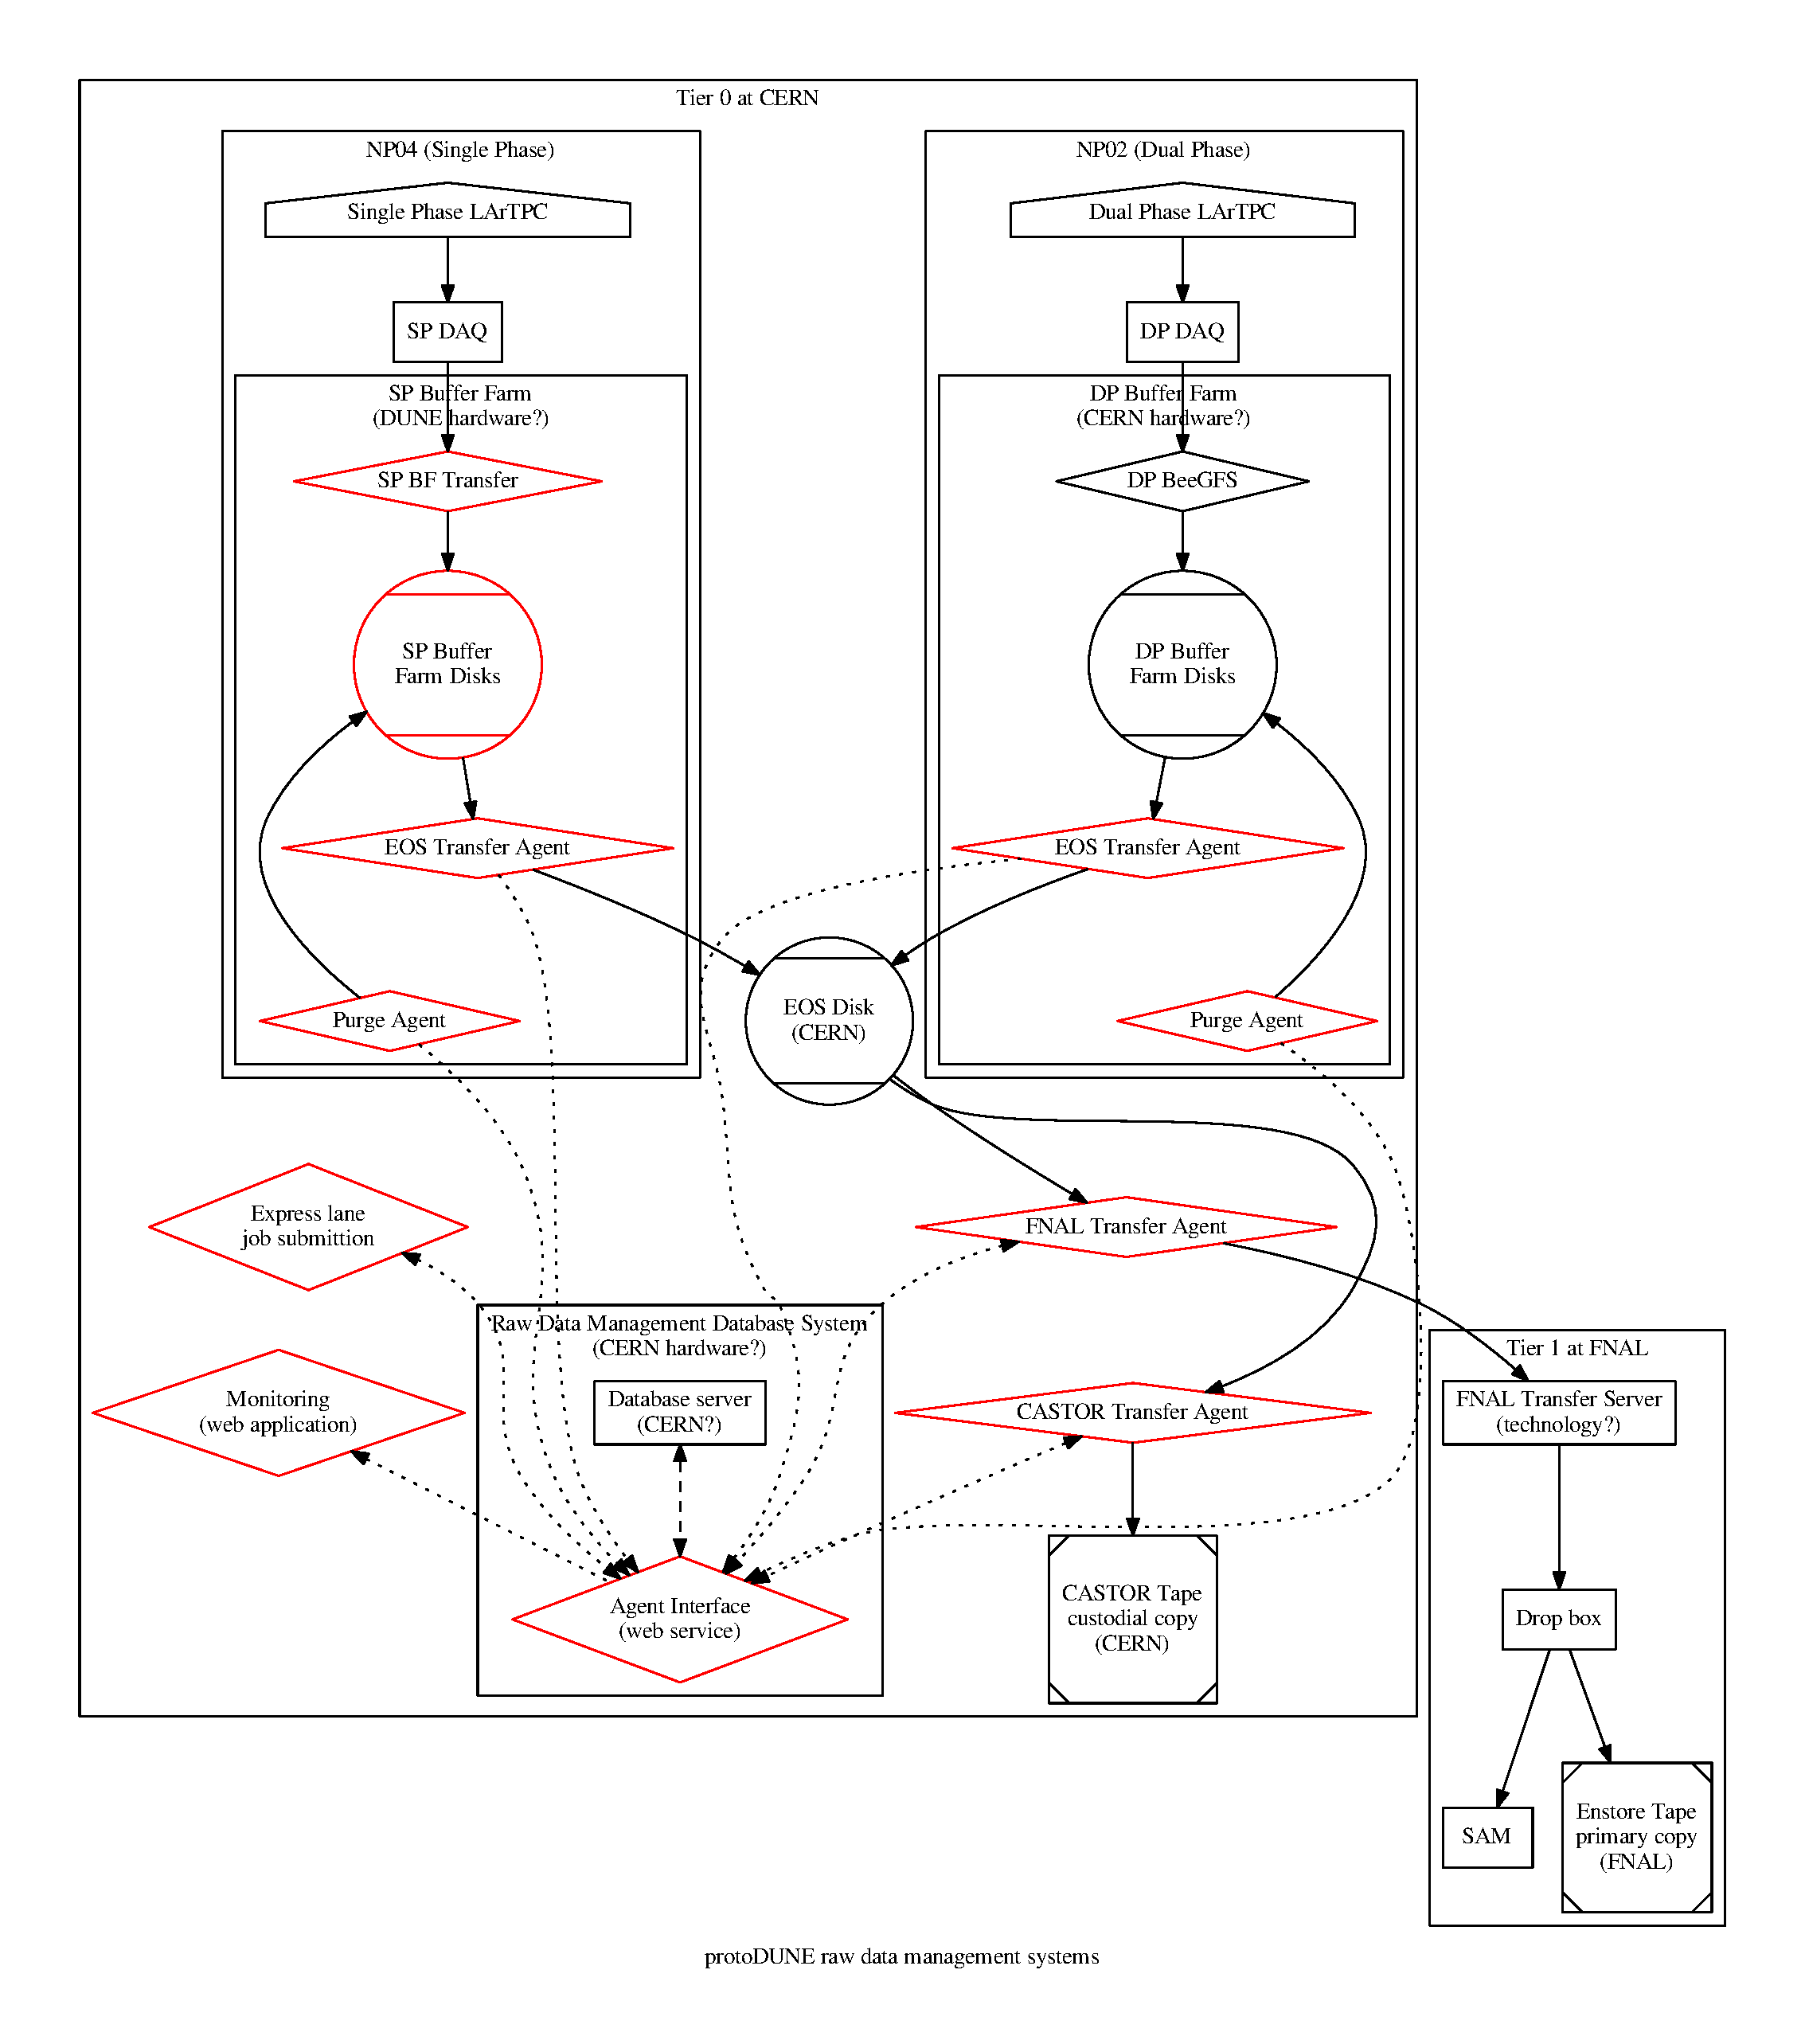
\includegraphics[width=0.8\textwidth]{flow.pdf}
%  \caption{Systems required for protoDUNE raw data management. }
%  \label{fig:flow}
%\end{figure}


\section{Hardware Systems}

\subsection{Buffer Farms}

It is assumed that each prototype detector has a nearby and dedicated
\textit{disk buffer farm} (BF).  They are required in order to isolate
online systems from offline ones.  Each BF is not necessarily expected
to be identical in terms of hardware characteristics or its software
because the two DAQs differ.  Their individual characteristics are:

\begin{description}
\item[DP buffer farm] requires \fixme{XXX} TB distributed on
  \fixme{XXX} computer nodes with \fixme{XXX} bandwidth.  It is
  provided by \fixme{CERN(?)}.
\item[SP buffer farm] requires \fixme{XXX} TB distributed over
  \fixme{XXX} nodes with \fixme{XXX} bandwidth.  It is provided by
  \fixme{DUNE(?)}.
\end{description}

As described more in section~\ref{subsec:eosxferagent}, it is expected
that starting from the buffer farms the handling of the data from each
detector source will be symmetric in terms of what systems are
employed.  Other differences such as data rates, total volume, format
must be accommodated.

\subsection{EOS and CASTOR}

The EOS disk and CASTOR tape systems are expected to be provided by
CERN.  DUNE must estimate the required volume and bandwidth into each
of these systems (and out of EOS) for each detector individually and
should then negotiate with CERN to understand what is needed for them
to provide that.  DUNE should formulate an internal policy and
mechanisms to assure proper storage management and sharing so that
data from both prototypes can be accommodated.

\subsection{FNAL Ingest and Enstore}

The protoDUNE raw data management system will assure the raw data
files successfully reach Fermilab's transfer server.  Another system
is expected to then assure the data is properly cataloged and archived
to FNAL Enstore tape.  It is expected the same systems used for DUNE
35t and other Fermilab-based experiments will be used.  Specifically
the transfer server will deposit the accepted raw data files into a
``drop box''.  From there any metadata about the file will be inserted
into the SAM databas and the file itself archived to Enstore.

\section{Software Systems}

\subsection{DAQ-BF Transfer systems}

Raw data must be transferred from each detector DAQ to its respective
BF disk storage.  The general requirements of the DAQ-BF transfer
system are:

\begin{itemize}
\item must scale to provide required level of throughput from DAQ to disk.
\item integrating into developed DAQ software must not require
  substantial new effort.
\item the DAQ must not block while a transfer is ongoing such that it
  can not accept new data from readout electronics.
\end{itemize}

The transfer systems for the two detectors may differ.  Current
understanding and recommendations are summarized:

\begin{description}
\item[dual-phase] The DP detector has selected BeeGFS~\cite{beegfs}
  distributed, network file system for transferring data from DAQ to
  buffer disks.  

\item[single-phase] The SP detector requires development or adoption
  of a transfer method.  It is recommended to evaluate the technology
  adopted by DP and to evaluate XrootD~\cite{xrootd}
\end{description}

It is with files appearing on the respective BF that the protoDUNE Raw
Data Management (RDM) system takes over the provenance of the raw data
files.

\subsection{Raw Data Management System}

The protoDUNE RDM system is based on the idea of each file progressing
through a state machine of well defined states and explicit
transitions between those states.  State transitions are enacted by a
set of software agents.  The agent is required to perform an action
based on the current state of a file as set in the central RDM
database and record the outcome of the transition in said database.

Most agents will be written to perform a number of state transitions.
Some may inject initial state based on external information (eg, a
file appearing on a BF).  Other agents may merely monitor state
changes.  Figure~\ref{fig:flow} describes one possible set of agents.
As we learn more the set may grow with new functionality or splitting
large agents into smaller ones.  These agents are described in
section~\ref{subsec:agents}.

\subsection{Database}

The database is required to:
\begin{description}
\item[performance] accept new records at a rate on order of 10Hz and
  read-only queries an order of magnitude higher.
\item[schema] full history of inserts (no update nor delete of a
  previously inserted row), generate a unique identifier for each managed
  raw data file, relational associations to that ID.
\end{description}
The database is not directly exposed to agents but instead an Agent
Interface (RDM AI) is provided as an HTTP ``web service'' API,
described next


\subsection{Agent Interface}

The only direct access to the database should be through the Agent
Interface.  It is required to:
\begin{itemize}
\item present all database operations through a HTTP ``web service'' API.
\item expose functionality required by all expected agents as described below.
\item support and require authentication/authorization where needed.
\end{itemize}

All clients of the database shall use this interface, be they actually
effecting state changes or be they merely monitoring the state of the
database.

\subsection{Agents}
\label{subsec:agents}

Agents are expected to be command line programs or in some cases web
applications.  In general, they are required to:

\begin{itemize}
\item access and authenticate to the RDM AI
\item respect the allowed state transitions
\item report back on the outcome
\end{itemize}



\subsubsection{EOS Transfer Agent}
\label{subsec:eosxferagent}

The EOS Transfer Agent (ETA) is responsible for transferring files
from the BFs to EOS and recording the results.  Some detail will be
given here as a prototype for what must be given for all agents.

\begin{figure}[h]
  \centering
  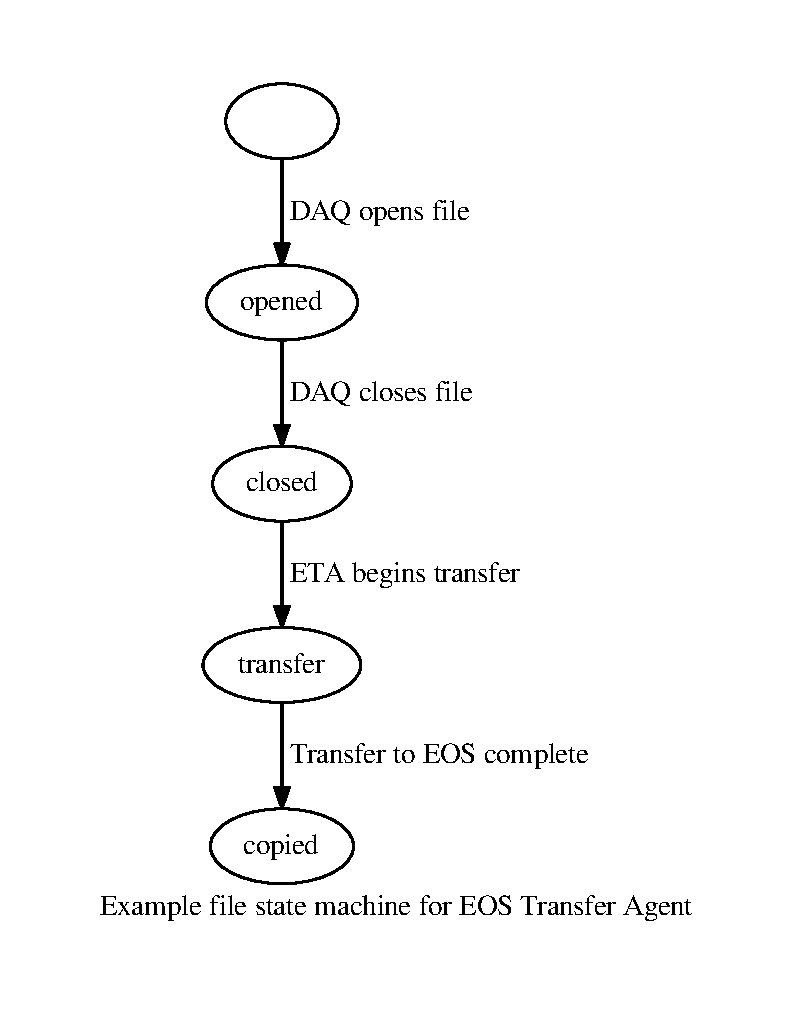
\includegraphics[width=0.5\textwidth]{state.pdf}
  \caption{EOS Transfer Agent states and transitions.}
  \label{fig:state}
\end{figure}

Figure~\ref{fig:state} gives the state machine implemented by the ETA.
This agent progresses sequentially through its possible states.  It
begins by watching its BF for the appearance of a new file and when
one appears it registers the file to the RDM DB via the AI that the
file is in state \texttt{opened}.  When it determines the DAQ has
finished writing the file this is registered as \texttt{closed} and a
transfer to EOS is begun with the equivalent \texttt{transfer} state
recorded.  When the transfer successfully concludes the
\texttt{copied} state is entered.

In addition to that behavior the ETA must
\begin{itemize}
\item be able to perform read and delete file operations on raw data
  files from both detectors BF disk storage
\item honor detector-specific policy regarding the timing of these
  file operations.
\item able to produce copies of raw files on EOS
\end{itemize}


\subsubsection{CASTOR Transfer Agent}

The CASTOR Transfer Agent (CTA) archives a file from EOS to CASTOR
tape.  It is required that the CTA:

\begin{itemize}
\item only archive a file that has reached the \texttt{copied} state
\item can read EOS file system and write to CASTOR
\end{itemize}

\subsubsection{Purge Agent}

The Purge Agent is responsible for deleting files when certain
conditions are met, depending on the context of the file to purge.
For example, BF files might only be purged after copied to EOS or they
may be delayed until archived to CASTOR.  A differently configured
Purge Agent may operate on files in EOS and purge based the file
reaching some appropriate state in the RDM DB.

\subsubsection{FNAL Transfer Agent}

The FNAL Transfer Agent (FTA) is responsible for transferring files
that have been copied to EOS to Fermilab via a to be determined
transfer server.  It is required to read EOS disk and connect to this
server.  

Once the transfer successfully complete, the fate of the raw file is
no longer the concern of the protoDUNE raw data management system.
Its continued management is taken over by systems at Fermilab.

\section{Summary and Future}

This report gives an outline for a design for a Raw Data Management
system for DUNE single-phase and dual-phase prototype detectors.  It
is based on agents enacting state changes on the files orchestrated by
a central database.  There are still many unknowns and gaps in the
design and it is expected that this document will be updated as the
design matures.  The design still needs to be presented to experts in
both SP and DP online, CERN and FNAL management and larger DUNE
collaboration.


\end{document}

%%% Local Variables:
%%% mode: latex
%%% TeX-master: t
%%% End:
